\documentclass[11pt]{article}

\usepackage[utf8]{inputenc}
\usepackage[T1]{fontenc}

\usepackage{fullpage}

\usepackage{graphicx}
\usepackage{verbatim}
\usepackage{siunitx}

\usepackage[colorlinks=false,pdfborder={0 0 0}]{hyperref}
\usepackage[all]{hypcap}


\title{Astro 585: HW 5}
\author{Codename: The Maxwell-Jüttner Distribution}



\begin{document}


\maketitle

My git repository is here: \url{https://github.com/hsgg/astro585}, clone URL
\url{https://github.com/hsgg/astro585.git}.


\section{Density Matrix}
This was done in pair coding.


\section{Lookup tables}
\verbatiminput{2.jl}

The simple graph for 2c:\\
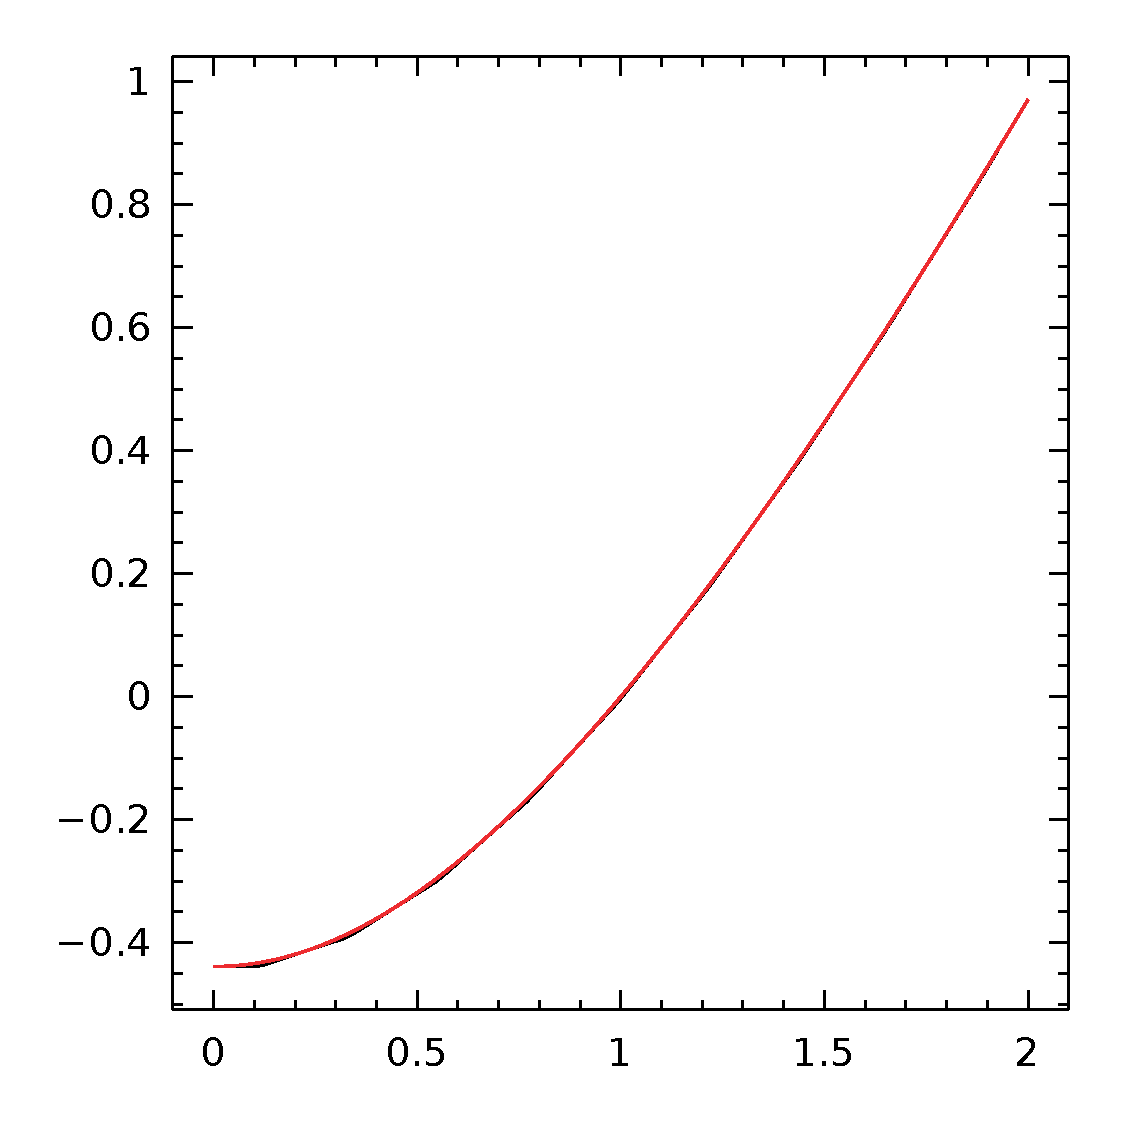
\includegraphics[width=0.5\textwidth]{2c_test.pdf}

ecc\_anom for 2d:\\
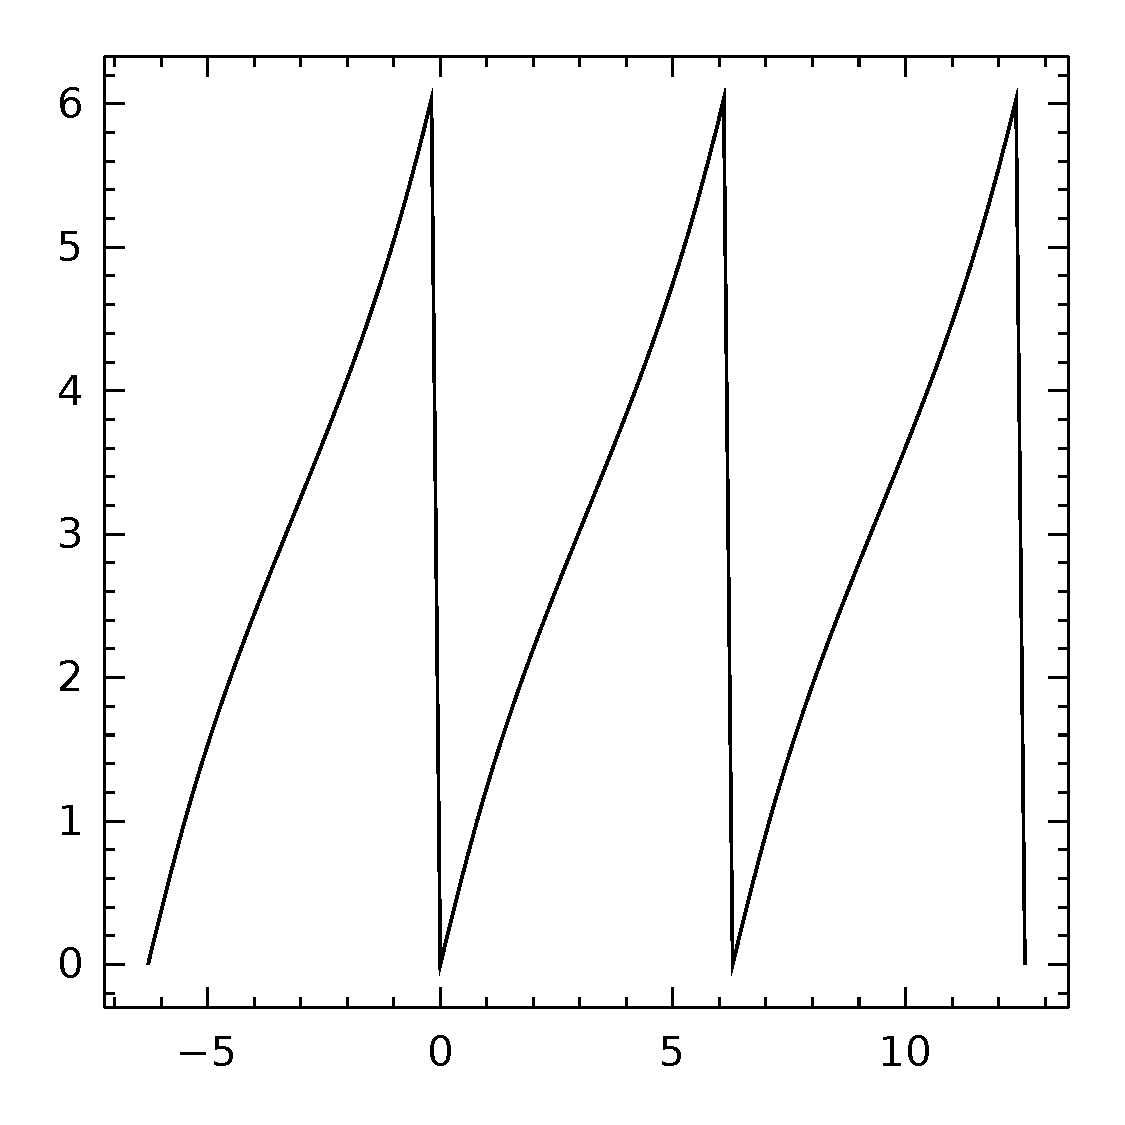
\includegraphics[width=0.5\textwidth]{2d_ecc_anom.pdf}

ecc\_anom for 2e, when it gets ugly:\\
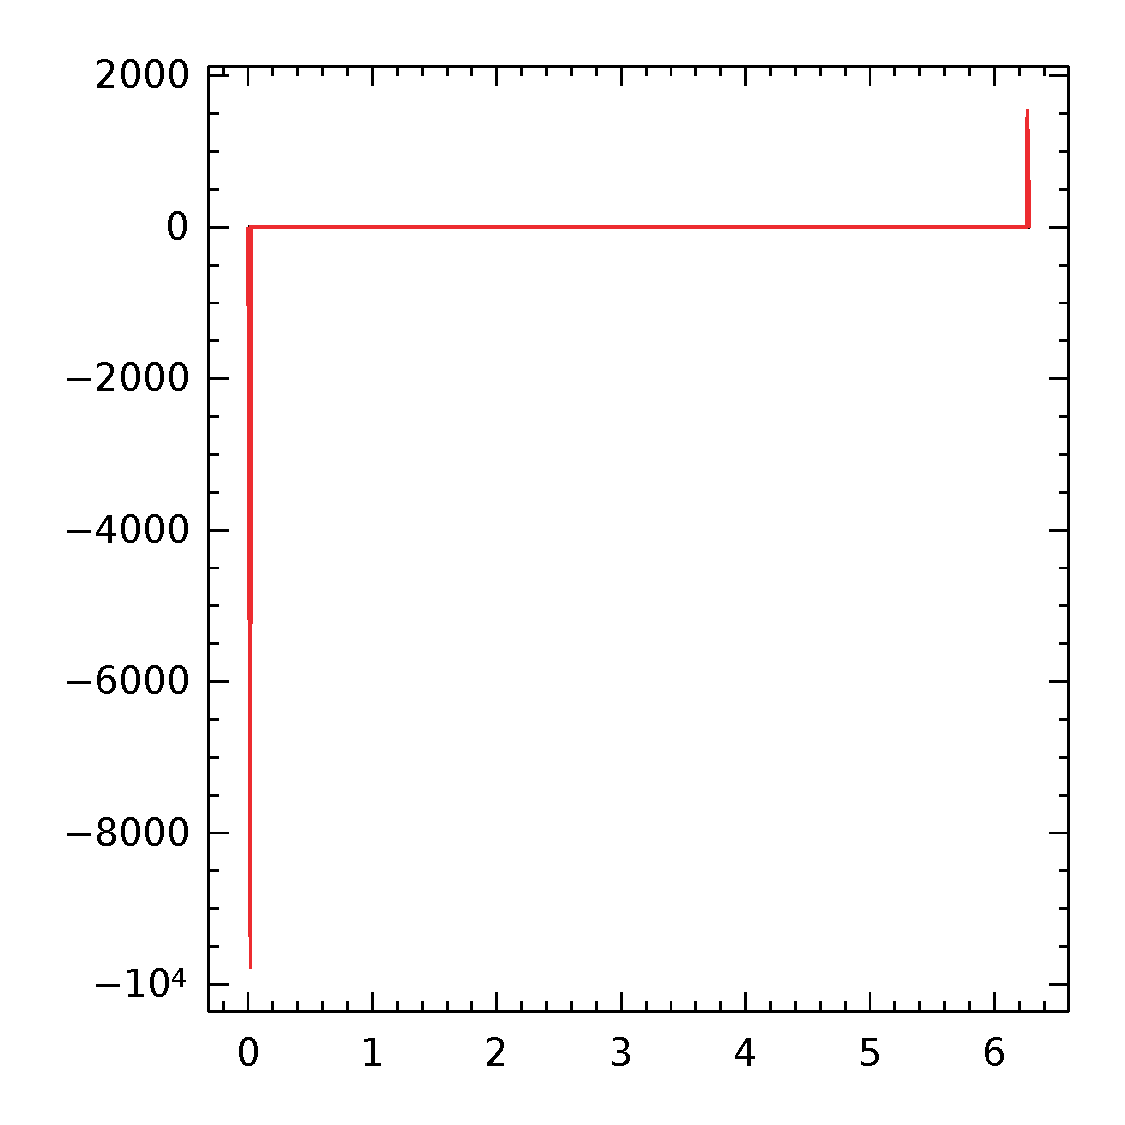
\includegraphics[width=0.5\textwidth]{2e_ecc_anom_poor.pdf}

ecc\_anom for 2f, when it remains ugly:\\
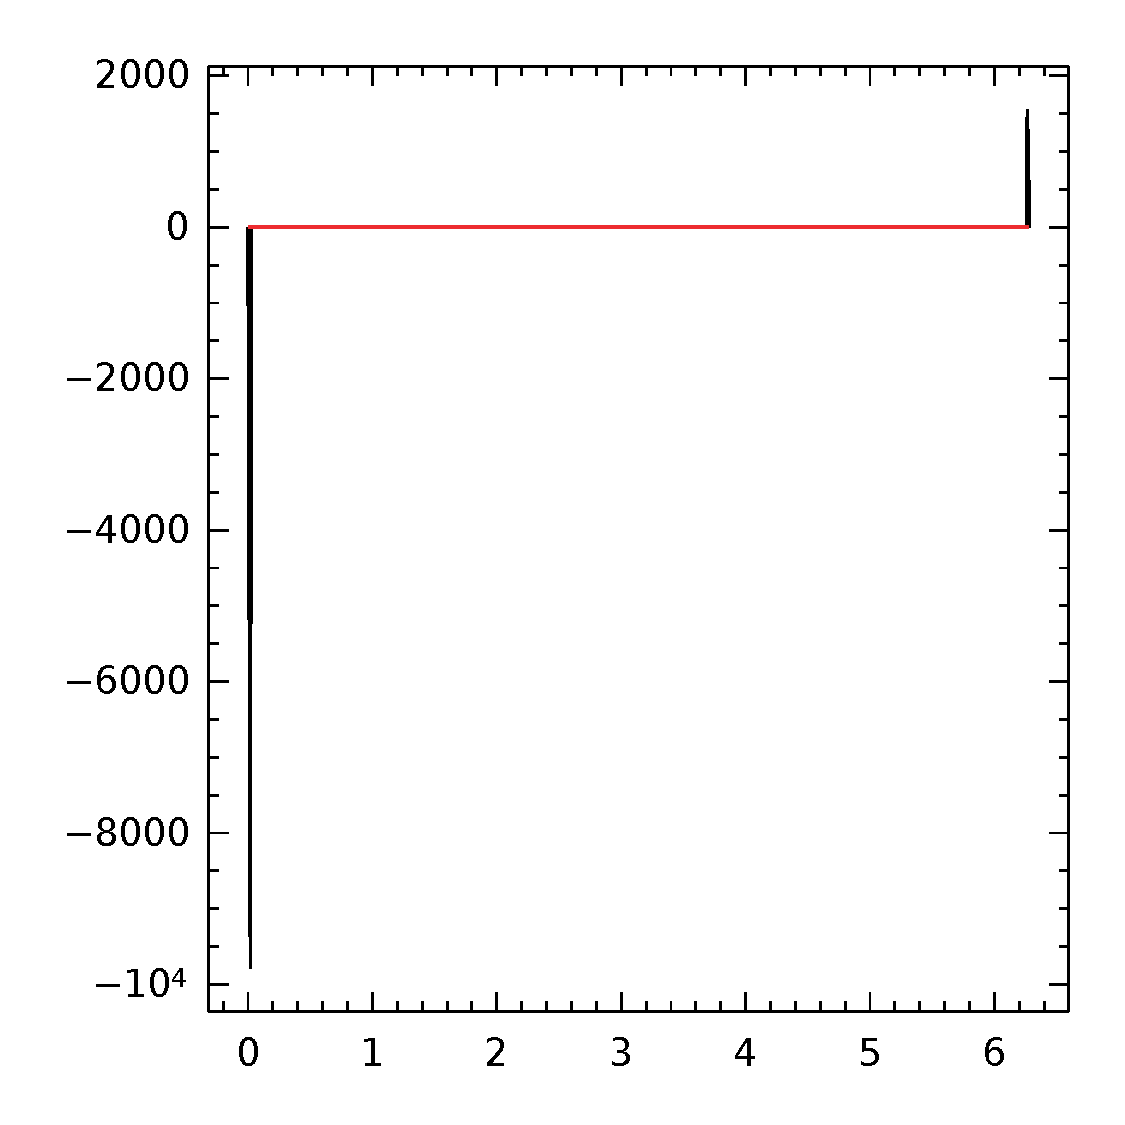
\includegraphics[width=0.5\textwidth]{2f_ecc_anom_stillpoor.pdf}

ecc\_anom for 2g, when it quadratic interpolation doesn't help:\\
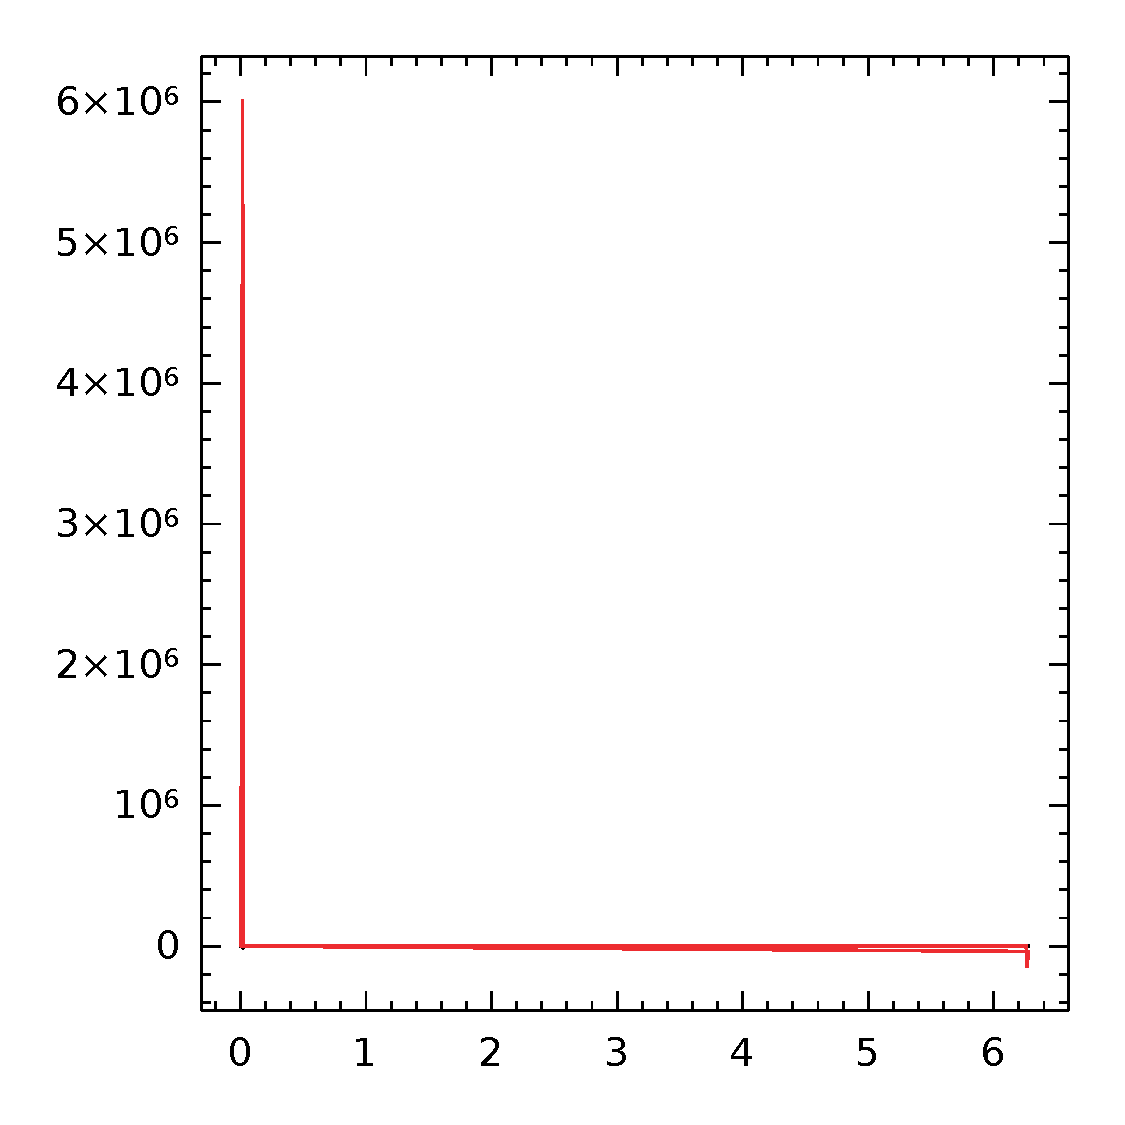
\includegraphics[width=0.5\textwidth]{2g_ecc_anom_stillpoor_quadratic.pdf}



\end{document}
